\documentclass[t]{beamer}\usepackage[]{graphicx}\usepackage[]{color}
%% maxwidth is the original width if it is less than linewidth
%% otherwise use linewidth (to make sure the graphics do not exceed the margin)
\makeatletter
\def\maxwidth{ %
  \ifdim\Gin@nat@width>\linewidth
    \linewidth
  \else
    \Gin@nat@width
  \fi
}
\makeatother

\definecolor{fgcolor}{rgb}{0.345, 0.345, 0.345}
\newcommand{\hlnum}[1]{\textcolor[rgb]{0.686,0.059,0.569}{#1}}%
\newcommand{\hlstr}[1]{\textcolor[rgb]{0.192,0.494,0.8}{#1}}%
\newcommand{\hlcom}[1]{\textcolor[rgb]{0.678,0.584,0.686}{\textit{#1}}}%
\newcommand{\hlopt}[1]{\textcolor[rgb]{0,0,0}{#1}}%
\newcommand{\hlstd}[1]{\textcolor[rgb]{0.345,0.345,0.345}{#1}}%
\newcommand{\hlkwa}[1]{\textcolor[rgb]{0.161,0.373,0.58}{\textbf{#1}}}%
\newcommand{\hlkwb}[1]{\textcolor[rgb]{0.69,0.353,0.396}{#1}}%
\newcommand{\hlkwc}[1]{\textcolor[rgb]{0.333,0.667,0.333}{#1}}%
\newcommand{\hlkwd}[1]{\textcolor[rgb]{0.737,0.353,0.396}{\textbf{#1}}}%

\usepackage{framed}
\makeatletter
\newenvironment{kframe}{%
 \def\at@end@of@kframe{}%
 \ifinner\ifhmode%
  \def\at@end@of@kframe{\end{minipage}}%
  \begin{minipage}{\columnwidth}%
 \fi\fi%
 \def\FrameCommand##1{\hskip\@totalleftmargin \hskip-\fboxsep
 \colorbox{shadecolor}{##1}\hskip-\fboxsep
     % There is no \\@totalrightmargin, so:
     \hskip-\linewidth \hskip-\@totalleftmargin \hskip\columnwidth}%
 \MakeFramed {\advance\hsize-\width
   \@totalleftmargin\z@ \linewidth\hsize
   \@setminipage}}%
 {\par\unskip\endMakeFramed%
 \at@end@of@kframe}
\makeatother

\definecolor{shadecolor}{rgb}{.97, .97, .97}
\definecolor{messagecolor}{rgb}{0, 0, 0}
\definecolor{warningcolor}{rgb}{1, 0, 1}
\definecolor{errorcolor}{rgb}{1, 0, 0}
\newenvironment{knitrout}{}{} % an empty environment to be redefined in TeX

\usepackage{alltt}

\usetheme{Madrid}
\usecolortheme{seahorse}

\usepackage{geometry}
\usepackage{graphicx}
\usepackage{amssymb}
\usepackage{epstopdf}
\usepackage{amsmath}  	% this permits text in eqnarray among other benefits
\usepackage{color}          	% gives color options
\usepackage{url}		% produces hyperlinks
\usepackage[english]{babel}
\usepackage[latin1]{inputenc}
\usepackage{colortbl}	% allows for color usage in tables
\usepackage{multirow}	% allows for rows that span multiple rows in tables
\usepackage{xcolor}		% this package has a variety of color options
\usepackage{calc}
\usepackage{multicol}

\setbeamertemplate{navigation symbols}{}

%User defined colors: See colors section
\xdefinecolor{oiBlue}{rgb}{0.15, 0.35, 0.55}
\xdefinecolor{gray}{rgb}{0.5, 0.5, 0.5}
\xdefinecolor{darkGray}{rgb}{0.3, 0.3, 0.3}
\xdefinecolor{darkerGray}{rgb}{0.2, 0.2, 0.2}
\xdefinecolor{rubineRed}{rgb}{0.89,0,0.30}
\xdefinecolor{linkCol}{rgb}{0.11,0.49,0.95}	
\xdefinecolor{irishGreen}{rgb}{0,0.60,0}	
\xdefinecolor{darkturquoise}{rgb}{0.44, 0.58, 0.86}
\definecolor{lightGreen}{rgb}{0.533,0.765,0.42}

\setbeamercolor*{palette primary}{fg=white,bg= oiBlue!70}
\setbeamercolor*{palette secondary}{fg=black,bg= oiBlue!20!white}
\setbeamercolor*{palette tertiary}{fg=white,bg= oiBlue!80!black!90}
\setbeamercolor*{palette quaternary}{fg=white,bg= oiBlue}

\setbeamercolor{structure}{fg= oiBlue}
\setbeamercolor{frametitle}{bg= oiBlue!70}

\setbeamercolor{disc body}{bg=oiBlue!20!white!80,fg=oiBlue!80!black!90}
\setbeamercolor{disc title}{bg=oiBlue!40!white!60,fg=oiBlue!70!black!100}


\setbeamertemplate{blocks}[shadow=false]


\newcommand{\removepagenumbers}{% 
  \setbeamertemplate{footline}{
    %
    \begin{beamercolorbox}[colsep=1.5pt]{upper separation line foot}
    \end{beamercolorbox}
    \begin{beamercolorbox}[ht=2.5ex,dp=1.125ex,%
      leftskip=.3cm,rightskip=.3cm plus1fil]{author in head/foot}%
      \leavevmode{\usebeamerfont{author in head/foot}\insertshortauthor}%
%      \hfill%
%      {\usebeamerfont{author in head/foot}\usebeamercolor[fg]{institute in head/foot}\insertshortinstitute}%
    \end{beamercolorbox}%
    \begin{beamercolorbox}[ht=2.5ex,dp=1.125ex,%
      leftskip=.3cm,rightskip=.3cm plus1fil]{title in head/foot}%
      {\usebeamerfont{title in head/foot}\insertshorttitle}%
      \hfill%
      {\usebeamerfont{author in head/foot}\usebeamercolor[fg]{institute in head/foot}\insertshortinstitute}%
    \end{beamercolorbox}%
    \begin{beamercolorbox}[colsep=1.5pt]{lower separation line foot}
    \end{beamercolorbox}
    }
} 


\newcommand{\disc}[2]{
\begin{beamerboxesrounded}[shadow = true, lower = disc body, upper = disc title]{#1}
#2
\end{beamerboxesrounded}
}


\AtBeginSection[] 
{ 
  \addtocounter{framenumber}{-1} 
  % 
  {\removepagenumbers 
    \begin{frame}<beamer> 
    \tableofcontents[currentsection] 
  \end{frame} 
  } 
} 

\usepackage{bm}
\usepackage{isotope}
\usepackage{appendixnumberbeamer}

\newcommand{\PM}{$\text{PM}_{2.5}$ }

\title[Speciated \PM]{A Data Fusion Approach for Space-Time Analysis of Speciated \PM}
\author{Colin Rundel}
\date{August 3, 2014}
\institute[Duke]{Duke University}
\IfFileExists{upquote.sty}{\usepackage{upquote}}{}
\begin{document}

\begin{frame}[plain]
\titlepage
\end{frame}



%==================================================================================================

\begin{frame}
\frametitle{Background}
    
Fine particulate matter (\PM{}) is an EPA regulated air pollutant linked to a variety of adverse health effects

\begin{itemize}
  \vspace{2mm} \item Classified based on particle size ($<2.5$ $\mu$m diameter)
  \vspace{2mm} \item Major species: Sulfate, Nitrate, Ammonium, Soil, Carbon.
  \vspace{2mm} \item Minor species: trace elements (K, Mg, Ca), heavy metals (Cu, Fe), etc.
  \vspace{2mm} \item Complex spatio-temporal dependence between species
\end{itemize}


\end{frame}

%==================================================================================================

\begin{frame}
\frametitle{Data (2007)}

Speciated \PM Sources
\begin{itemize}
  \item Chemical Speciation Network (CSN) - 221 stations
  \item Interagency Monitoring of Protected Visual Environments (IMPROVE) - 172 stations
\end{itemize}

\vspace{2mm}

Total \PM Sources
\begin{itemize}
  \item Federal Reference Method (FRM) - 949 stations
\end{itemize}

\vspace{2mm}

Model Output
\begin{itemize}
  \item Community Multi-scale Air Quality (CMAQ) - 12 km grid
\end{itemize}

\vspace{5mm}

Data Issues
\begin{itemize}
  \item Monitoring frequency
  \item Total vs Sum of Species
\end{itemize}

\end{frame}


%==================================================================================================

\begin{frame}[t]
\frametitle{Total \PM vs Sum of Species}

\vfill

\begin{center}
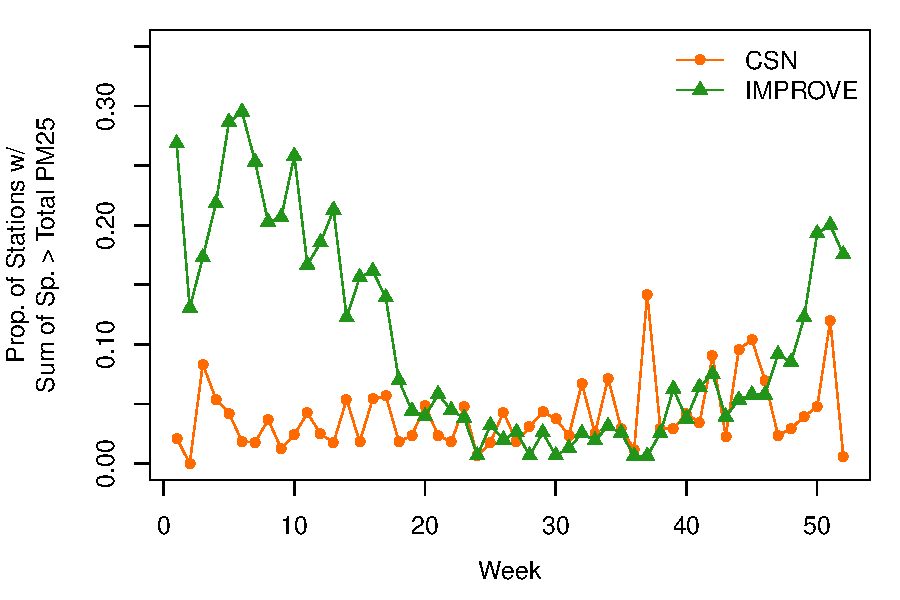
\includegraphics[width=0.9\textwidth]{figs/pm_exceed.pdf}
\end{center}

\vfill
	
\end{frame}

%==================================================================================================

\begin{frame}
\frametitle{Species Model Details}

For the 5 major species (Sulfate, Nitrate, Ammonium, Soil, Carbon) and the two networks (CSN, IMPROVE):
%
\begin{align*}
C_t^i(\bm{s}) &= Z_t^i(\bm{s}) + \epsilon_{C,t}^i(\bm{s}) \\
I_t^i(\bm{s}) &= Z_t^i(\bm{s}) + \epsilon_{I,t}^i(\bm{s})
\end{align*}

where $Z_t^i(\bm{s})$ are the latent ``true'' concentrations of species $i$ at time $t$ and locations $\bm{s}$,
%
\begin{align*}
{Z}_t^i(\bm{s}) &= \max{}\left(0,~\widetilde{Z}_t^i(\bm{s})\right) \\
\widetilde{Z}_t^i(\bm{s}) &= \beta_{0,t}^i +\beta_{0,t}^i(\bm{s}) + \beta_{1,t}^i \: Q_t^i(B_{\bm{s}})  
\end{align*}


\end{frame}

%==================================================================================================

\begin{frame}
\frametitle{Total \PM Model Details}

For total \PM from the three networks (CSN, IMPROVE, FRM):
%
\begin{align*}
C_t^{tot}(\bm{s}) &= Z_t^{tot}(\bm{s}) + \epsilon_{C,t}^{tot}(\bm{s}) \\
I_t^{tot}(\bm{s}) &= Z_t^{tot}(\bm{s}) + \epsilon_{I,t}^{tot}(\bm{s}) \\
F_t^{tot}(\bm{s}) &= Z_t^{tot}(\bm{s}) + \epsilon_{F,t}^{tot}(\bm{s})
\end{align*}

where $Z_t^{tot}(\bm{s})$ are the latent ``true'' concentration of total \PM at time $t$ and locations $\bm{s}$, which is given by the sum of the major species and the ``other'' species concentrations.
%
\[ Z^{tot}_{t}(\bm{s}) = \sum_{i=1}^{5} Z^i_t(\bm{s}) + Z^{o}_{t}(\bm{s}) \]

{\footnotesize
\[
{Z}_t^o(s) = \max{}\left(0,~\widetilde{Z}_t^o(s)\right) \qquad
\widetilde{Z}_t^{o}(\bm{s}) = \beta_{0,t}^o +\beta_{0,t}^o(\bm{s}) + \beta_{1,t}^o \: Q_t^o(B_{\bm{s}})
\]
}

\end{frame}

%==================================================================================================

\begin{frame}
\frametitle{Spatial Dependence}

Spatial dependence enters the model through the $\beta_{0,t}^i(s)$ parameters for $i \in \{o,1,2,3,4,5\}$.

\[ \beta_{0,t}^i(\bm{s}) = {\sigma}^i_t~w^i_t(\bm{s}) \]

\vspace{5mm}

where $w^i_{t}(\bm{s})$ are zero mean, variance $1$, Gaussian processes with exponential correlation given by 

\begin{align*}
\text{corr}(w^i_{t}(\bm{s}),w^i_{t}(\bm{s}')) = \exp(-\phi^i_{t} |\bm{s}-\bm{s}'|)
\end{align*}


\end{frame}

%==================================================================================================

\begin{frame}
\frametitle{Model results}

\vfill
\begin{center}
\vspace{-5mm}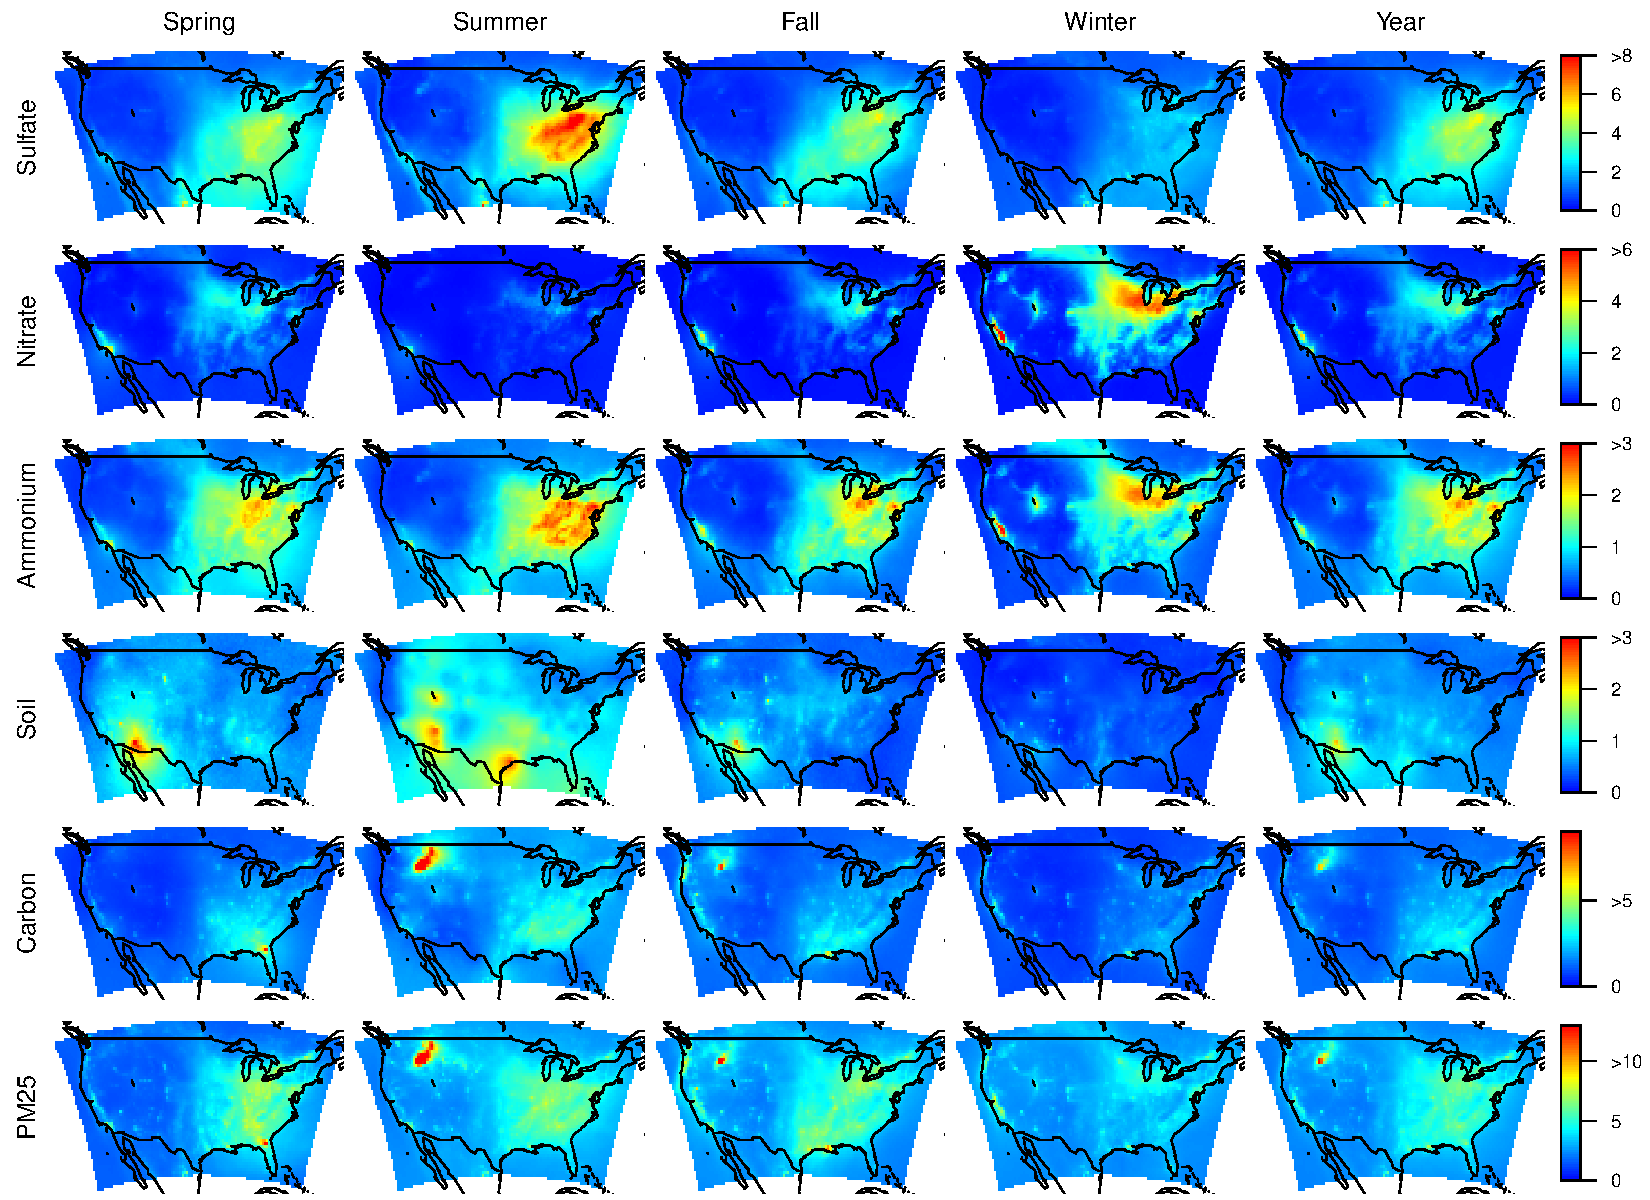
\includegraphics[width=0.9\textwidth]{figs/pm_maps.pdf}
\end{center}
\vfill

\end{frame}


%==================================================================================================

\begin{frame}
\frametitle{Model results}

\vfill
\begin{center}
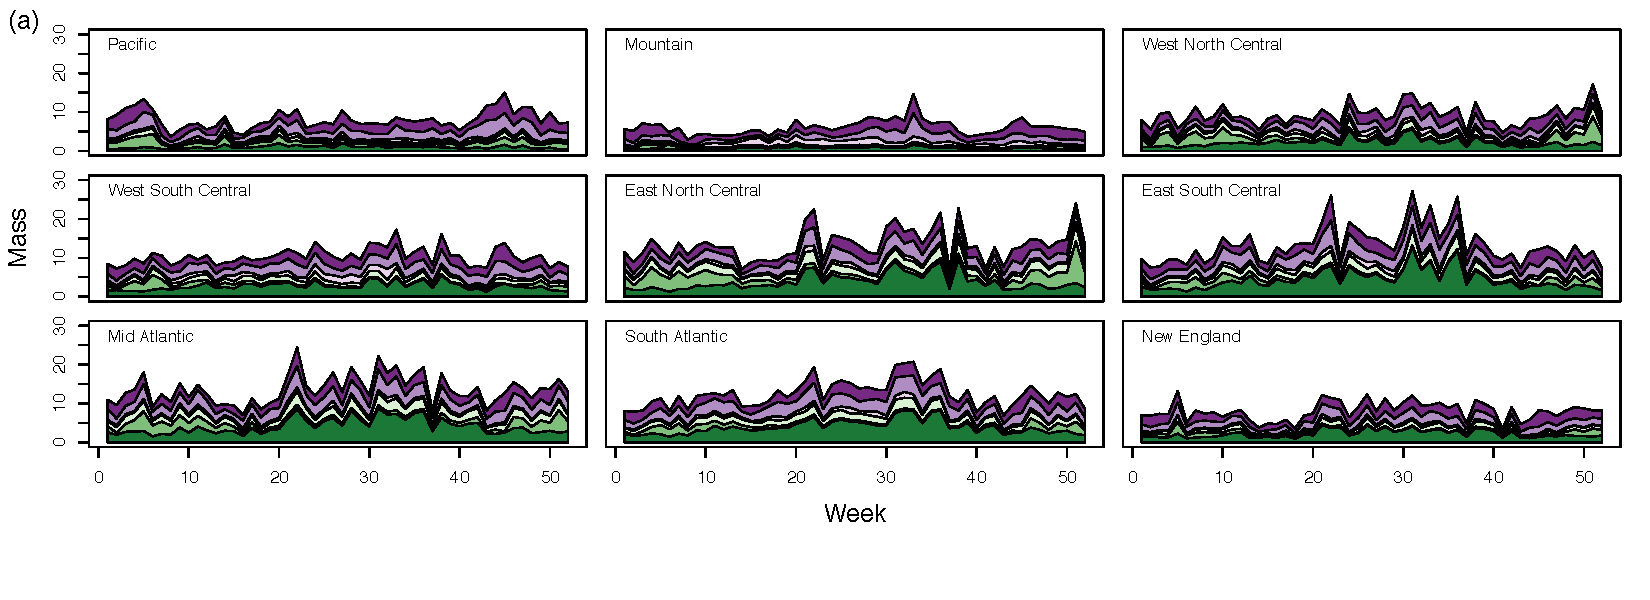
\includegraphics[width=\textwidth]{figs/pm_ts.pdf}\\
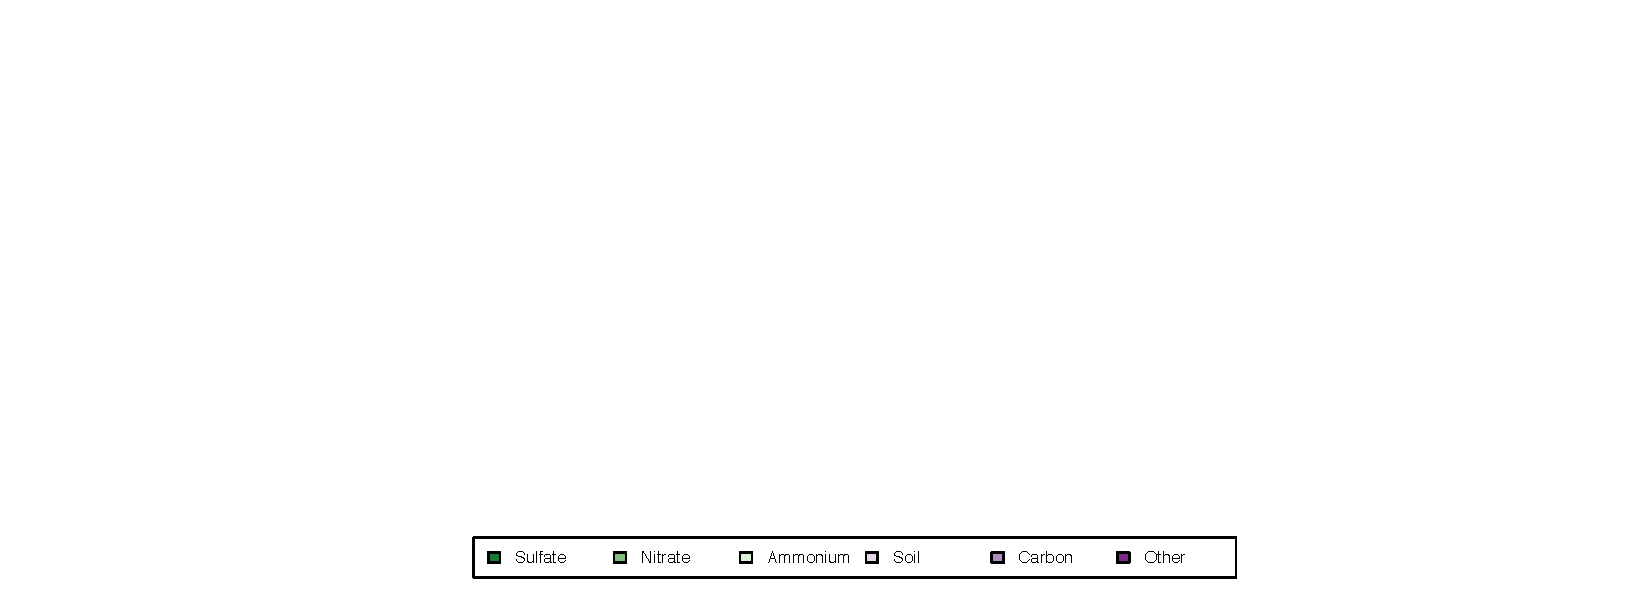
\includegraphics[width=\textwidth]{figs/pm_ts_legend.pdf}
\end{center}
\vfill

\end{frame}

%==================================================================================================

\begin{frame}
\frametitle{Model Validation}

\vfill

{\footnotesize
\begin{center}
\renewcommand*{\arraystretch}{1.5}
\begin{tabular}{l|l|cccccc}
    & & Sulfate & Nitrate & Ammonium & Soil & Carbon & PM25 \\
\hline
\parbox[t]{2mm}{\multirow{2}{*}{\rotatebox[origin=c]{90}{RMSE}}}
%%%
& Tobit w/o CMAQ & 1.347 & 2.257 & 0.858 & 1.363 & 3.073 & 6.298 \\
& Tobit          & 1.151 & 1.641 & 0.724 & 1.307 & 2.851 & 5.393  \\
%%%
\hline
\parbox[t]{2mm}{\multirow{2}{*}{\rotatebox[origin=c]{90}{CRPS}}}
%%%
& Tobit w/o CMAQ & 0.639 & 0.758 & 0.374 & 0.468 & 1.064 & 3.023  \\
& Tobit          & 0.554 & 0.558 & 0.329 & 0.438 & 0.885 & 2.452  \\
%%%
\hline
\parbox[t]{2mm}{\multirow{2}{*}{\rotatebox[origin=c]{90}{EmpCov}}}
%%%
& Tobit w/o CMAQ & 0.935 & 0.931 & 0.933 & 0.907 & 0.923 & 0.924  \\
& Tobit          & 0.920 & 0.930 & 0.924 & 0.915 & 0.921 & 0.906  \\
%%%
\hline
\end{tabular}
\end{center}
}

\vfill\vfill

Validation based on randomly selecting 10\% of stations as hold outs.

\end{frame}

%==================================================================================================

\begin{frame}
\frametitle{Run times}

Total run time for model fitting (50,000 iterations): \\ \vspace{2mm}

\begin{columns}[c]
\column{0.5\textwidth}
\begin{itemize}
\item CPU - 7.7 hours
\item CPU+GPU - 4.8 hours
\end{itemize}
\column{0.5\textwidth}
$\times$ 52 weeks
\end{columns}


\vfill


Total run time for model prediction at 5950 locations (1,000 iterations): \\ \vspace{2mm}

\begin{columns}[c]
\column{0.5\textwidth}
\begin{itemize}
\item CPU - 7.2 hours
\item CPU+GPU - 4.3 hours
\end{itemize}
\column{0.5\textwidth}
$\times$ 52 weeks
\end{columns}

\vfill

One run takes about 775 hours total on CPU alone, 473 on CPU and GPU.

\end{frame}

%==================================================================================================

\begin{frame}
\frametitle{Model fitting performance}

\begin{center}
\renewcommand*{\arraystretch}{1.5}
\begin{tabular}{c|c|c|c}
Parameter                 & CPU (secs) & CPU+GPU (secs)  & Rel. Performance \\
\hline           
$\beta_0, \; \beta_1$     & 0.00029    & 0.00030         & 0.97 \\
$\beta_0(s) $             & 0.09205    & 0.09132         & 1.00 \\
$\sigma$                  & 0.00383    & 0.00385         & 0.99 \\
$\phi$                    & 0.46084    & 0.25174         & 1.83 \\
$\epsilon$                & 0.00003    & 0.00003         & 1.00 \\
\hline
Total                     & 0.55708    & 0.34729         & 1.60
\end{tabular}
\end{center}

\end{frame}

%==================================================================================================

\begin{frame}
\frametitle{Acknowledgments}

\vfill


\begin{itemize}
  \item Alan Gelfand - Duke
  \vspace{3mm} \item Dave Holland - EPA
  \vspace{3mm} \item Erin Schliep - Duke
  \vspace{3mm} \item Wyat Apel - NERL
\end{itemize}


\vfill

{\footnotesize
Disclaimer - The U.S. Environmental Protection Agency through its Office of Research and Development partially collaborated in this research. Although it has been reviewed by the Agency and approved for publication, it does not necessarily reflect the Agency's policies or views.
}
\end{frame}

%==================================================================================================

\begin{frame}
\frametitle{Information \& Questions}

\vfill

\begin{center}
{\Large
\renewcommand*\arraystretch{1.5}
\begin{tabular}{llp{8cm}}
Email        & : & {\normalsize rundel@gmail.com} \\
Presentation & : & {\normalsize \url{http://github.com/rundel/Presentations/}} \\
Paper        & : & {\footnotesize Rundel C., Schliep E., Holland D., Gelfand A. (2014)
                                  A data fusion approach for space-time analysis of speciated PM2.5.
                                  \textit{The Annals of Applied Statistics}. \textit{In submission}}
\end{tabular}
}
\end{center}

\vfill

\pause

\begin{center}
{\Large Questions?}
\end{center}

\vfill

\end{frame}

%==================================================================================================

\appendix

%==================================================================================================

\begin{frame}
    


\end{frame}

%==================================================================================================


\begin{frame}
\frametitle{Performance}

\vfill

\begin{columns}[t]
\column{0.6\textwidth}
System Specs:
\vspace{2.5mm}
\begin{itemize}
\item 4 core Intel i5-2500K @ 3.30 GHz
\vspace{2mm} \item 16 GB DDR3 @ 1333 MHz
\vspace{2mm} \item GeForce GTX 460
\end{itemize}

\column{0.4\textwidth}
Software Specs:
\vspace{0.5mm}
\begin{itemize}
\item Ubuntu 13.10
\vspace{2mm} \item OpenBlas 0.2.8
\vspace{2mm} \item CUDA 6.0RC
\vspace{2mm} \item Magma 1.4.1
\end{itemize}
\end{columns}

\vfill

\end{frame}

%==================================================================================================

\begin{frame}[label=univ]
\frametitle{Species Distributions}

\vfill
\begin{center}
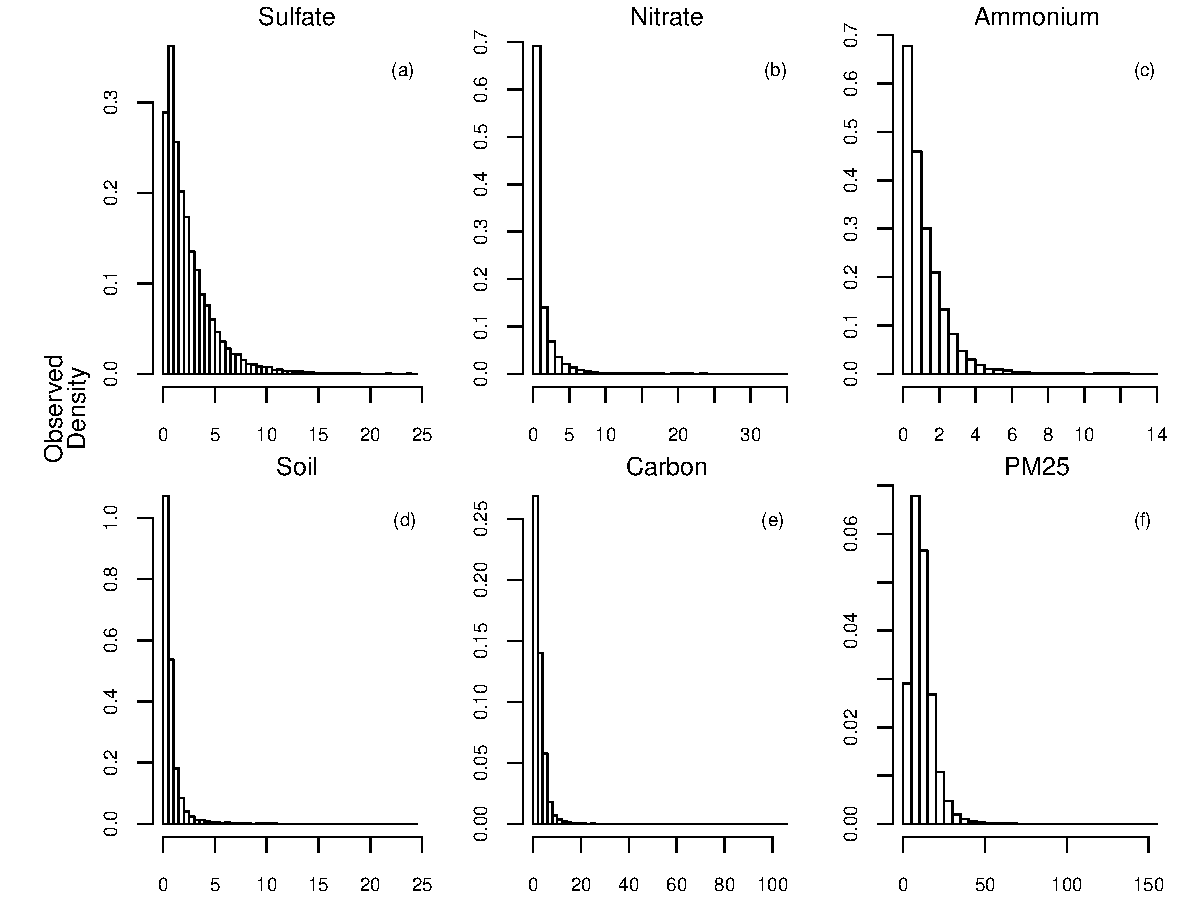
\includegraphics[width=0.8\textwidth]{figs/pm_hists.pdf}
\end{center}
\vfill

\end{frame}

%==================================================================================================

\begin{frame}[label=univ]
\frametitle{Univariate Model Exceedance}

\vfill
\begin{center}
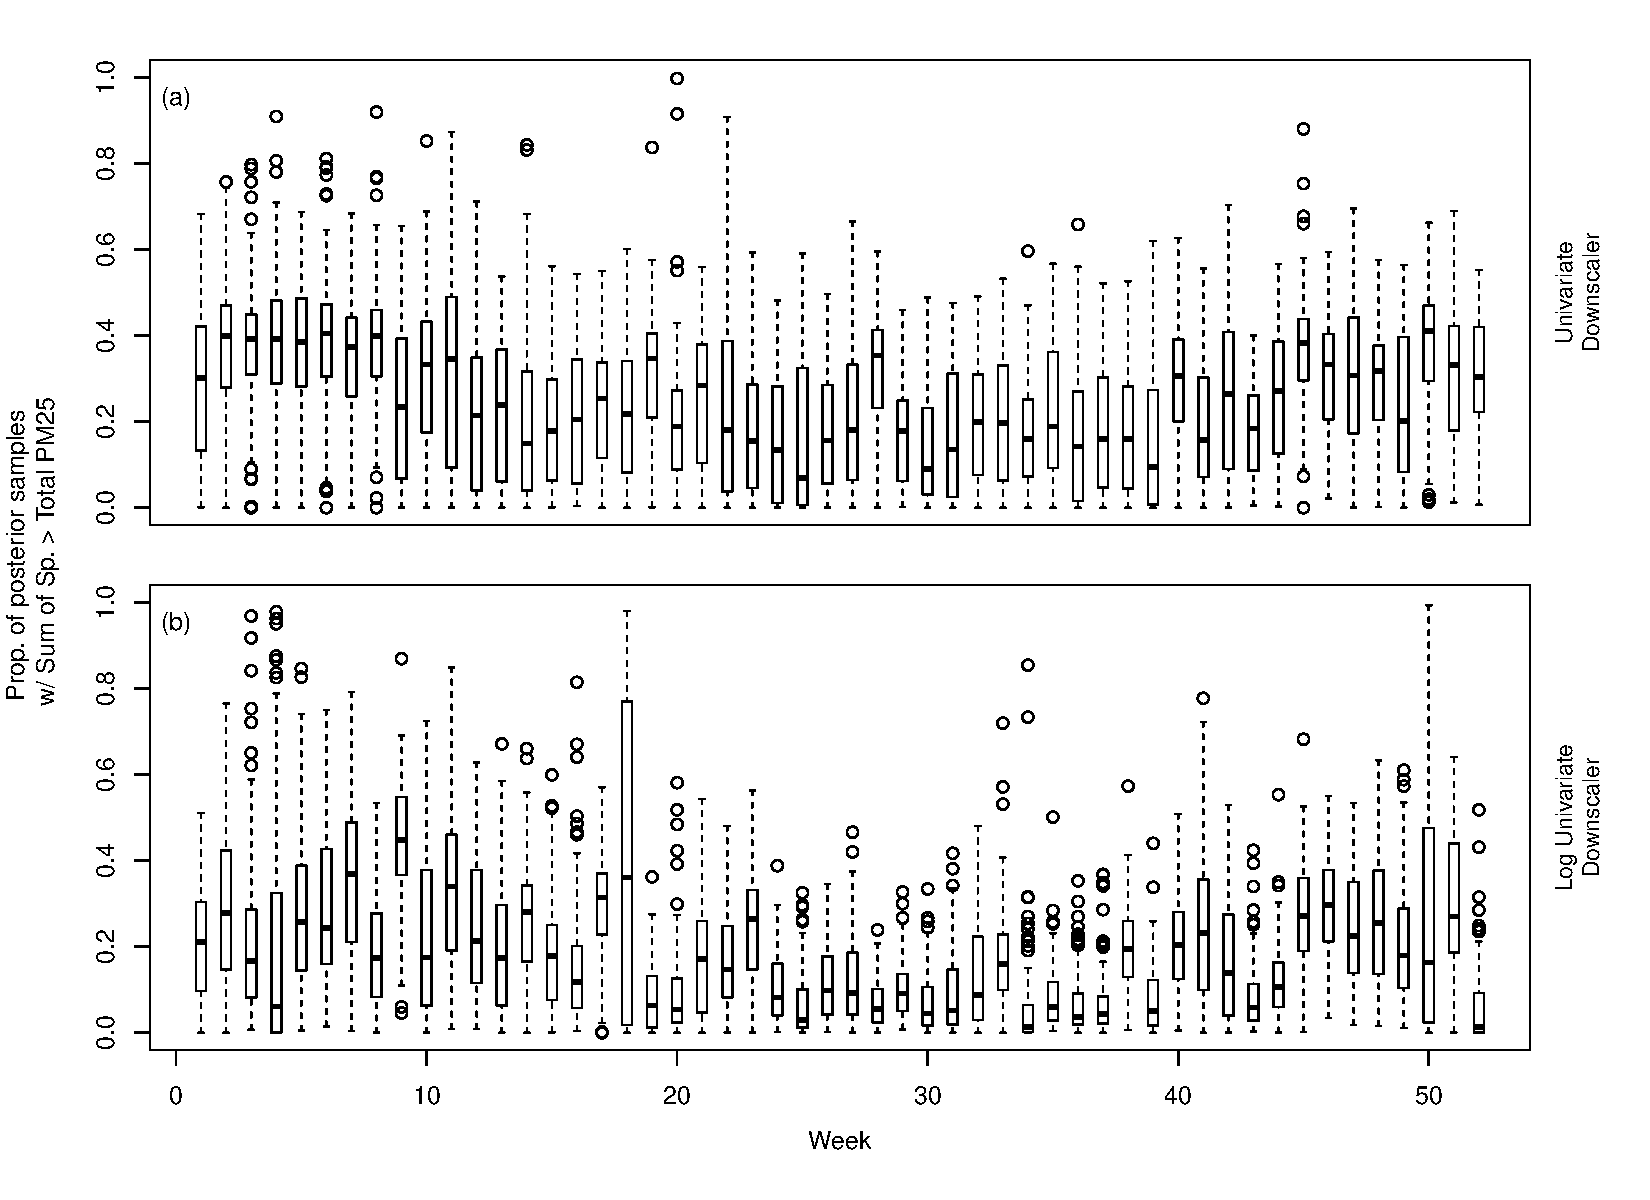
\includegraphics[width=0.9\textwidth]{figs/pm_exceed_uni.pdf}
\end{center}
\vfill

\end{frame}

%==================================================================================================


\begin{frame}[label=cmaq]
\frametitle{CMAQ Maps}

\vfill
\begin{center}
\vspace{-4mm}
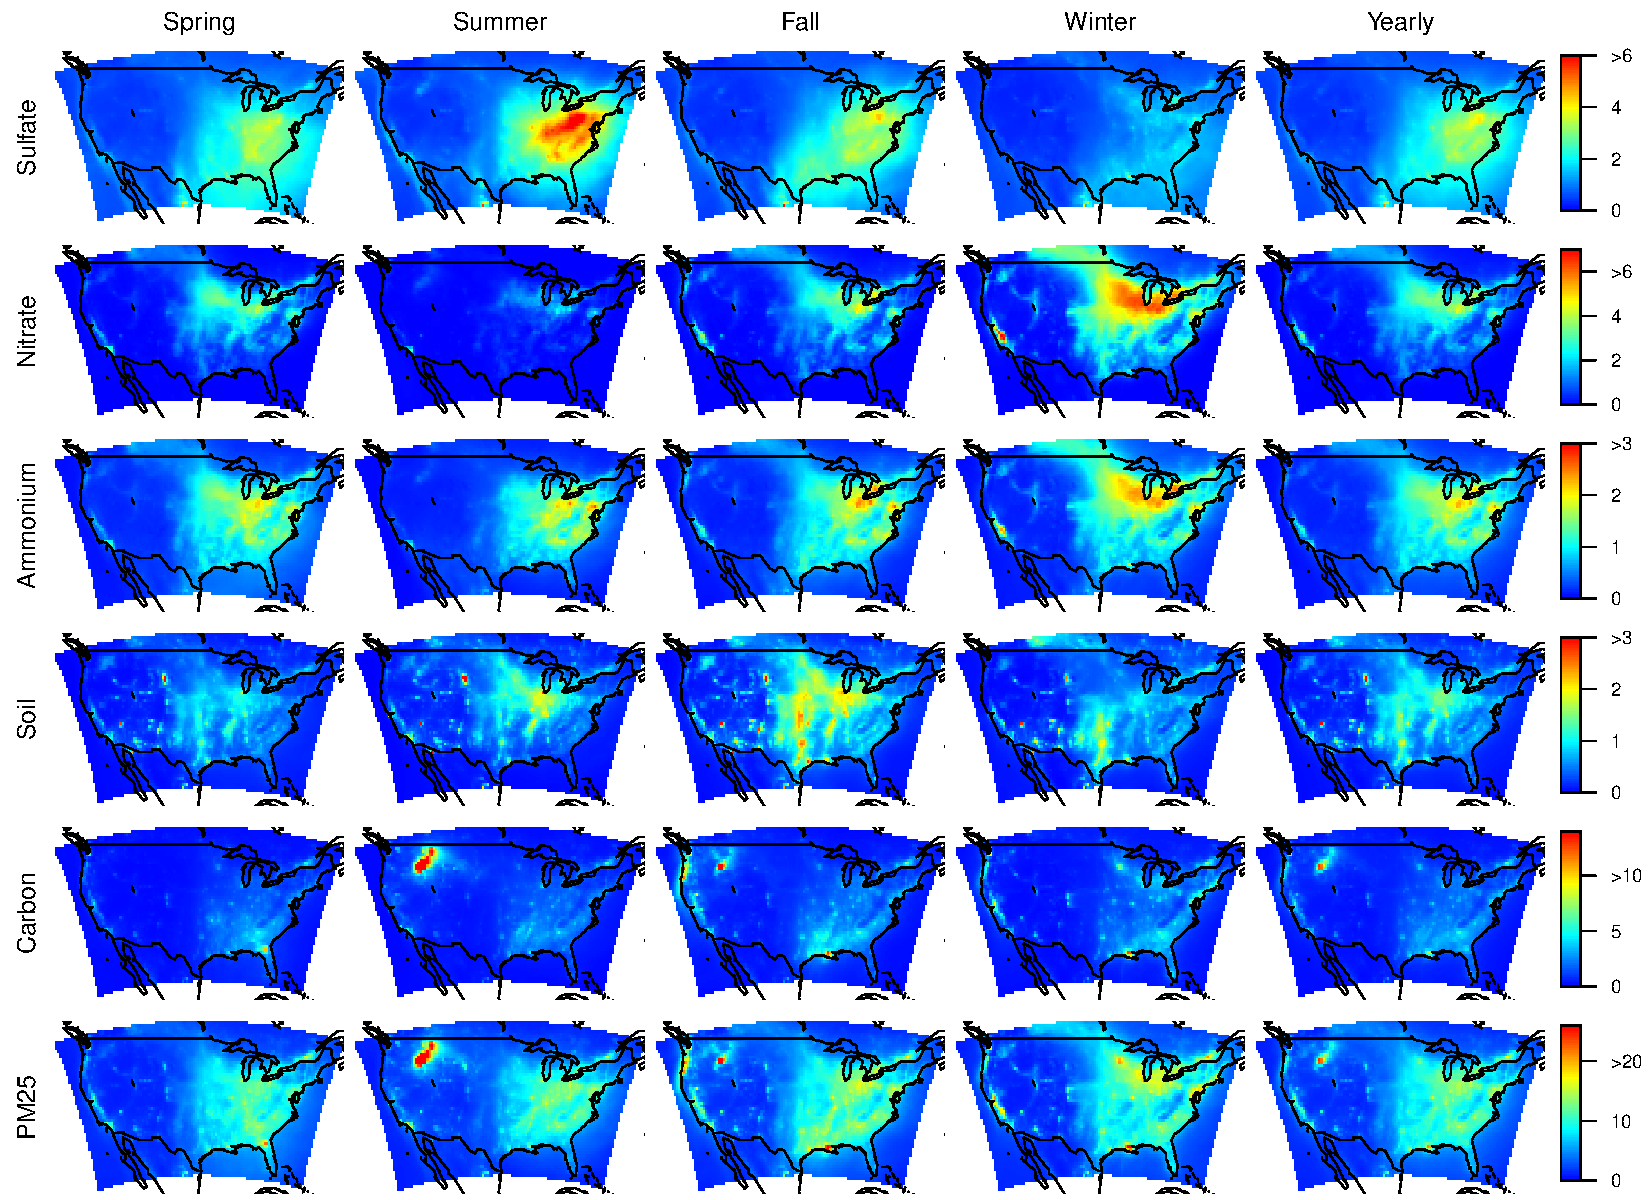
\includegraphics[width=0.9\textwidth]{figs/pm_maps_cmaq.pdf}
\end{center}
\vfill

\end{frame}


%==================================================================================================

\begin{frame}
\frametitle{Data TS}

\vfill
\begin{center}
\vspace{-4mm}
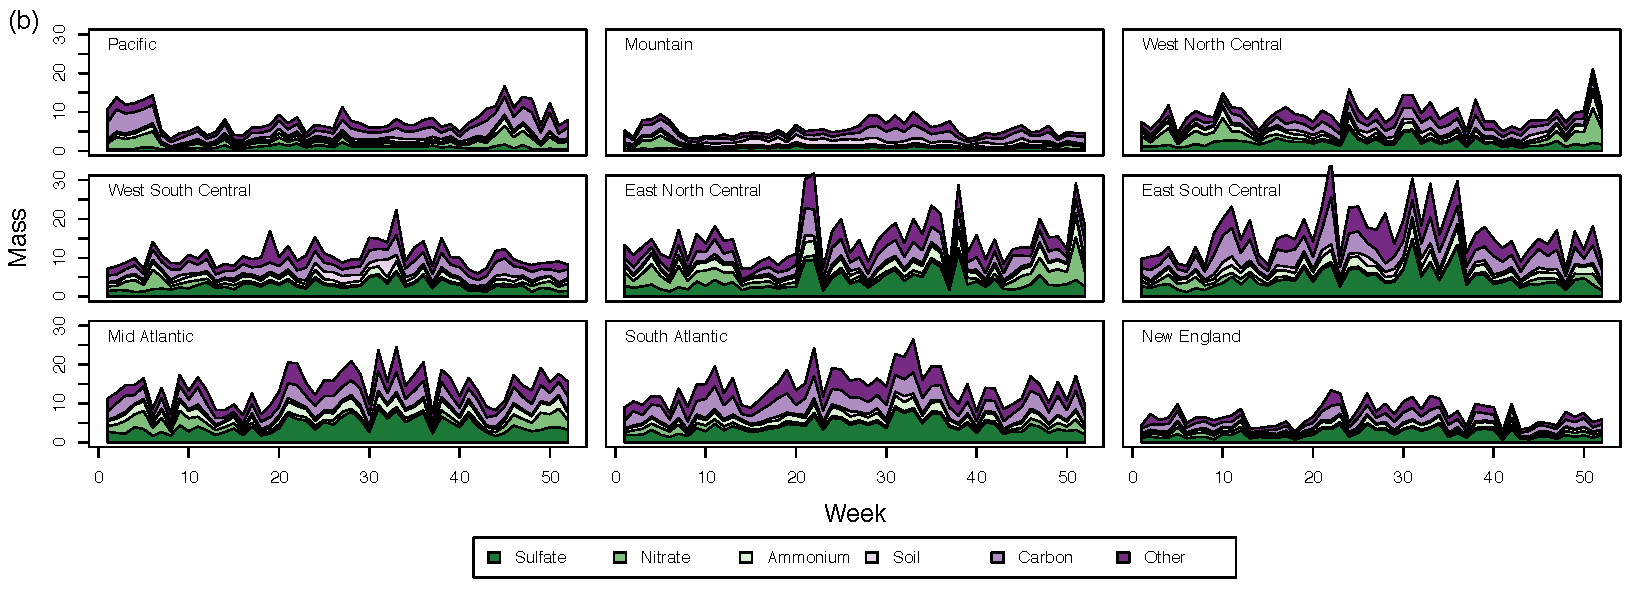
\includegraphics[width=0.9\textwidth]{figs/pm_ts_data.pdf}
\end{center}
\vfill

\end{frame}


%==================================================================================================


\begin{frame}[label=regions]
\frametitle{Regions}

\vfill
\begin{center}
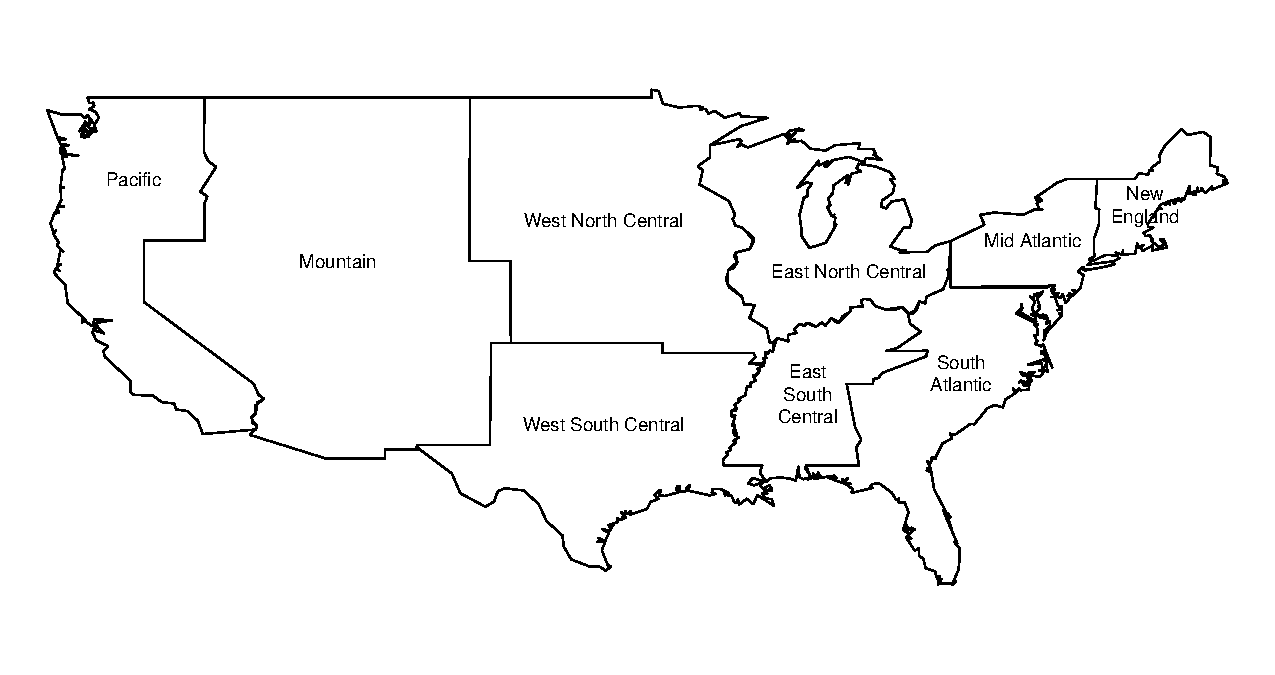
\includegraphics[width=0.9\textwidth]{figs/pm_regions.pdf}
\end{center}
\vfill

\end{frame}

\end{document}
